\documentclass[12pt]{article}
\usepackage[utf8]{inputenc}
\usepackage{bera}
\usepackage{geometry}
\geometry{a4paper, portrait, margin=1.1in}
\usepackage{graphicx}
\usepackage{amsmath}
\usepackage{blkarray}
\usepackage[noeepic]{qtree}
\usepackage{todonotes}
\renewcommand{\labelitemi}{$\bullet$}
\begin{document}
 \begin{titlepage} 
 \centering     
 \vspace*{3.5cm}         
 
     \vspace*{2.4cm}     
 
     \Huge \textbf{Software Lab: InLab\\Advanced \LaTeX}     
 
     \vspace*{0.8cm}     
 
     \LARGE{Pm9}
     
     \large{19305R009}

     \large{193050055}
     
     \large{193050023}
     \vspace*{0.5cm}     
 
     \large{28st August, 2019}     
     \vspace*{4.0cm}     
 
     \vspace*{\fill} 
 \end{titlepage}

 \setcounter{page}{1} 
 \tableofcontents 
 
 \clearpage

\section{Itemize, Enumerate and Description}
\subsection{Itemize}
\begin{itemize}
\item \LaTeX{} typesets a file of text using the TEX program
\item \LaTeX{} is widely used in academia for the communication and publication of scientific documents in many fields, including mathematics, physics, computer science, statistics, economics and political science.
\item \LaTeX{} can be used as a standalone document preparation system or as an intermediate format
\item \textbf{Have used renewcommand for the bullets to be bigger.}
\end{itemize}

\subsection{Enumerate}
\begin{enumerate}
\item \LaTeX{} typesets a file of text using the TEX program.
\item \LaTeX{} is widely used in academia for the communication and publication of scientific documents in many fields, including mathematics, physics,
computer science, statistics, economics and political science.
\item \LaTeX{} can be used as a standalone document preparation system or as an intermediate format.
\item \LaTeX{} is intended to provide a high-level language that accesses the power of TeX in an easier way for writers.
\end{enumerate}

\subsection{Description}
\begin{description}
\item[$\bullet$ Red] A colour at the end of the spectrum next to orange and opposite violet, as of blood, fire, or rubies. program.
\item[$\bullet$ Blue] A colour intermediate between green and violet, as of the sky or sea on a sunny day.
\item[$\bullet$ White] The colour of milk or fresh snow, due to the reflection of all visible rays of light; the opposite of black.
\item[$\bullet$ Black] The darkest colour owing to the absence of or complete absorption of light; the opposite of white.
\end{description}

\newpage
\section{Mathematical formulas and notations}

\subsection{Matrix}
Adjacency matrix of corresponding graph.

\medskip

\begin{center}
\begin{tabular}{r|l}
     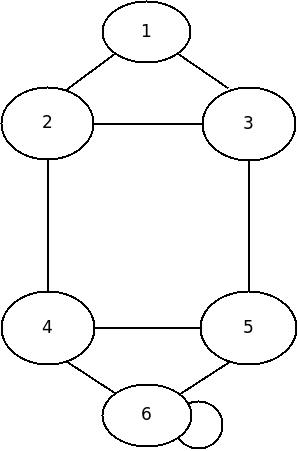
\includegraphics[width=4cm,height=5cm]{diagramSection2.jpeg}
     &
     \begin{blockarray}{ccccccc}
         & \textbf{1} & \textbf{2} & \textbf{3} & \textbf{4} & \textbf{5} & \textbf{6} \\
     \begin{block}{c(cccccc)}
     \textbf{1} & 0 & 1 & 1 & 0 & 0 & 0 \\
      \textbf{2} & 1 & 0 & 1 & 1 & 0 & 0 \\
      \textbf{3} & 1 & 1 & 0 & 0 & 1 & 0 \\
      \textbf{4} & 0 & 1 & 0 & 0 & 1 & 1 \\
      \textbf{5} & 0 & 0 & 1 & 1 & 0 & 1 \\
      \textbf{6} & 0 & 0 & 0 & 1 & 1 & 2 \\
     \end{block}
     \end{blockarray}
\end{tabular}
\end{center}

\subsection{Equation Array}

\begin{align}
    \cos{2\theta} &= \cos^2{\theta} - \sin^2{\theta} \\
    &= 2\cos^2{\theta} - 1
\end{align}
        
\subsection{Prepositional Formulae using Various Operators}
\vspace{0.5cm}
\begin{math}
    \neg(\forall{x})(\boldsymbol{\varphi}(x)) \longleftrightarrow (\exists{x})\neg\boldsymbol{\varphi}(x)
    \\[10pt]
    (\forall{x}(\boldsymbol{\psi}{x}\boldsymbol{\Lambda\psi}{x})) \longleftrightarrow ((\forall{x})\boldsymbol{\varphi}(x)\boldsymbol{\Lambda}(\forall{x})\boldsymbol{\varphi}(x))
\end{math}

\hspace{0cm}

\begin{center}
\begin{tabular}{|c|c|}
    \hline
   Greek Letters:  &  
   $\alpha A \beta B \gamma \Gamma \rho \rho P \sigma \Sigma \delta \Delta \varepsilon \varepsilon E$
   \\ 
	& \\
   \hline
\end{tabular}
\end{center}

\subsection{Mathematical Formulas}

\begin{math}
    1.\hspace*{0.2cm} \frac{\pi}{4} = \sum\limits_{n=0}^{\infty} \frac{(-1)^n * \overbrace{(1+1+\cdots+1)}^{n} }{(2n+1)*n}
\end{math}


\newpage
\section{Quote}

\subsection{Quote}
The margins of the quote environment are indented on both the left and the
right. The text is justified at both margins. Leaving a blank line between text
produces a new paragraph.The package csquotes offers a multilingual solution
to quotations, with integration to citation mechanisms offered by BibTeX.
\begin{center}

\setlength{\leftskip}{1cm}
\setlength{\rightskip}{1cm}

{“Unlike the quotation environment, paragraphs are not indented. It’s important to remark that even if you are typing quotes on English there are different quotation marks used in English (UK) and English (US).”}

\setlength{\leftskip}{0cm}
\setlength{\rightskip}{0cm}

\end{center}

\section{Algorithm and Pseudo Code}
\subsection{Tabbing}

//Breadth First Search Function\\
void BFS(list<longlong int> queue,long long int length)\\
\hspace*{1cm}long long int v;\\
\hspace*{1cm}if(queue.empty())\\
\hspace*{2cm}return;\\
\hspace*{1cm}list<long long int>::iterator i;\\
\hspace*{1cm}list<long long int> queue temp;\\
\hspace*{1cm}while(!queue.empty())\{\\
\hspace*{2cm}v=queue.front();\\
\hspace*{2cm}queue.pop front();\\
\hspace*{2cm}for(i=adj[v].begin();i!=adj[v].end();i++)\{\\
\hspace*{3cm}if(!pro ver[*i])\{\\
\hspace*{4cm}result[*i]=length;\\
\hspace*{4cm}queue temp.push back(*i);\\
\hspace*{4cm}pro ver[*i]=true;\\
\hspace*{4cm}adj[*i].remove(v);\\
\hspace*{3cm}\}\\
\hspace*{2cm}\}\\
\hspace*{1cm}\}\\
\hspace*{1cm}BFS(queue temp,length+6);\\
\hspace*{0cm}\}\\

\newpage

\section{Tree}
This tree is not an image it is a LaTeX based tree funcation. Figure this out.\\
\newline
\Tree[.If-statement If exp \textit{then} [.S if exp \textit{then} S ] ]


\end{document}
